\chapter{Search Trees}
\label{ch:search-trees}

\section{Finding Things}

Consider the problem of keeping things organized so you can find them.
It's not hard if you don't have many things.
If you have a dozen pairs of socks, you can just throw them in a drawer
and find the pair you want quickly, without really having to search.
However, if you run an office supply store that carries thousands of
types of paper, envelopes, pencils, and erasers,
you'll need to arrange them carefully, so people can find them.

The importance of being organized increases with the number of items.
If you run a warehouse, you might have to keep track of many thousands of things.
One solution is to associate a stock number with each
kind of item, set up a bin for each, and arrange the bins by
\index{stock number search}stock number.
That works reasonably well, even if there are many thousands of kinds of items.
When the warehouse decides to stock a new kind of item, you just set up
a bin at the end of the line and give it a stock number higher than the
one before it.

However, what if an item gets discontinued?
You can empty out its bin, but what do you do with the space?
It might be okay to leave the space empty for the first few discontinuations,
but with many thousands of items, there will be, over time, thousands
of discontinuations, and you'll end up wasting a lot of space.

Furthermore, stock numbers solve the problem of finding the
right bin, but they don't solve the problem of remembering the stock number
that goes with, say, 20-pound, white paper versus color ink cartridges.
To be able to find the stock number associated with
an item, you'll need some kind of index that arranges the items in
categories, subcategories, and the like, and perhaps in alphabetical
order by name within each category.
When the warehouse discontinues an item,
you need to cross it out in the index,
and when a new kind of item comes in, you need to write it into
the index at the appropriate place.
Eventually, the index is a mess, and needs reprinting.

You might be able to make this work, even for many thousands of items,
but you can see that the idea doesn't scale up well, and when you're
trying to keep track of many millions of things, as you might need to
do, for example, if you were the data manager for a large company,
keeping lists in order by name or stock number becomes
untenable. New kinds of data need to be added every day, or even every
few seconds, and obsolete items need to be deleted.
So, keeping the items in a list starting with the first item,
then the second, third, and so on cannot work in practice.
It will require too much data movement to expand spaces between
items to insert new ones or collapse space between items to delete old ones.
The problem needs a better solution,
and that's what this chapter is about.
Let's recap the problem.

\emph{Pile of socks method}.
If you have only a few items to keep track of,
the \index{socks, pile of}\index{pile of socks}pile-of-socks method works.
When you get a new pair of socks, you just throw it in the drawer.
When an old pair wears out, you just throw it away.
If you want to locate a particular pair of socks,
you just look through the drawer,
pair by pair, until to find the one you're looking for.
If you have ten pairs, the first pair you look at might be
the one you want, or the second, or third.
At worst, you'll have to look through all ten pairs.
On average you'll probably find the right pair
after looking through about half of them.

\emph{Binary search method}.\label{binary-search-method}
If you had a thousand books on your bookshelves,
you could arrange them in alphabetical order by title.
When you get a new book, you just insert it in the right place,
maybe sliding a few books around to accommodate it.
If you lose one, you can just leave the slot empty,
or slide the books around to fill in the space.

To find a particular book, you would probably just guess about
where it would be, look there, and adjust your next guess accordingly.
However, there is an efficient way to manage your search that
guarantees finding it in just a few steps. It's called \emph{binary search}.
First, you look at the middle book.
If it's the one you want, great. You're done.
If not, the title you're looking for will either
come after the middle one or before it in alphabetical order.
In either case, the number of possibilities has been cut in half,
and you can repeat the procedure to find the book you're looking for
among the remaining possibilities.
Since you cut the number of books in half each time,
it will not take more than ten steps to locate
a particular book among a thousand books
because cutting 1,000 in half, then cutting 500 in half,
and so on, you get down to one in ten steps.

Looking at it from the other direction, starting from one
and doubling at each stage, it goes 1, 2, 4, 8, 16, 32, 64,
128, 256, 512, 1024. These are the powers of two:
$2^0$, $2^1$, $2^2$, $2^3$ \dots $2^{10}$.
So, the number of items you need to examine
in the binary search procedure
when there are $n$ items, altogether, is the
first integer $k$ that makes $2^k \geq n$, or
what amounts to the same thing, $k \geq log_2(n)$.
That is, the number of steps in a
\index{search!binary}\index{binary search}binary search through
$n$ items is \index{logarithm}$log_2(n)$ rounded up
to the next integer.

When you round a number up to the next integer, you get the
\index{ceiling brackets}\index{brackets!ceiling}\emph{ceiling}
of the number:
$\lceil x \rceil$ $=$ ceiling of $x$ $=$ $x$ rounded up to the next integer.
With this notation, the formula for the maximum number of steps
required to locate a particular item using
binary search with a collection of $n$ items
is $\lceil log_2(n) \rceil$.

This gives binary search an amazing
advantage in speed over the pile-of-socks method.
It reduces the number of steps required to find a particular item
in a collection of $n$ items from an average of $n/2$
in the pile-of-socks approach to
to a maximum of $\lceil log_2(n) \rceil$
using binary search.
That's $(n/2)/\lceil log_2(n) \rceil$ times faster,
and $(n/2)/\lceil log_2(n) \rceil$ turns
out to be a very big number when there are a lot of items.

\index{search!binary vs linear}For a thousand items,
binary search is, on the average,
$(1000/2)/\lceil log_2(1000) \rceil$ times faster than the pile-of-socks method.
That's about 50 times faster.
For a ten thousand items, it's 350 times times faster.
The speed-up factor rises to over 3,000 for a hundred thousand items,
and for a million items binary search is, on the average,
over 25,000 times faster than the pile-of-socks method.
It gets better and better the more items you have,
and in the computer search business, it is common to search for one item among
millions, billions, or even trillions of items.\footnote{For the record,
binary search is 17 million times faster for a billion items
and 12 billion times faster for a trillion items.
The pile-of-socks method would not be a feasible way
to find one item among billions if you had to make such a search
millions of times every day.}

So, binary search, or something as good or better, is indispensable.
The good news is that we can rely on it.
The bad news is that, while it works
well for a few thousand items, the problem of
keeping the items arranged in order
becomes unwieldy, to say the least, when there are
millions of items.

That's what happens when the items are entries in
an \index{search!array}\index{array!search}array of $n$ elements,
numbered, say, 0 to $n - 1$.
Whenever you add a new item or delete an old one,
you have to move things around, one way or the other,
to make space or fill in gaps to
keep the numbers that select array elements
in a contiguous sequence, 0, 1, 2, 3, \dots.
So, keeping items in order with indexes in sequence
to facilitate using binary search
works fine when the items don't change,
but becomes infeasible when they do.
In practice, items tend to come and go,
so we need to organize the items in some way
other than just numbering them sequentially.

\section{The AVL Solution}

Not long after computers began to have enough
memory to keep track of many thousands of items,
the mathematicians \index{Adelson-Velskii, Georgy}Adelson-Velskii
and \index{Landis, Evgenii}Landis
devised a structure that
eliminated the problem of sliding things around to
accommodate new items (the \emph{insertion problem})
or get rid of old ones (the \emph{deletion problem}).
This structure, known as the
\index{AVL tree}\index{binary tree!AVL}\index{tree!AVL}AVL tree
(``AV'' for Adelson-Velskii and ``L'' Landis)\label{AVL-tree},
makes it possible to find an item or
insert a new one
in only about $log(n)$ steps, where $n$ is the number
of items stored in the tree.
It takes about the same number of steps to delete an item,
so the AVL solution provides a practical way to do all three
operations: search, insertion, and deletion.
Adelson-Velskii and Landis solved a very difficult problem
when they figured out how to do this,
but their solution isn't hard to explain,
and that is the goal of this chapter.

We will need some terminology to discuss the idea.
\label{empty-tree-def}\index{tree!definition}The term \emph{tree}
will mean either an \emph{empty tree}
or a \label{node-def}\emph{node} called the
\label{root-def}\emph{root}.
A node consists of a sequence of one or more subtrees, and each
\label{subtree-def}\index{subtree, definition}\emph{subtree}
is also a tree.
That is, each subtree is either the empty tree
or a node, which is its root.\footnote{Yet
another usefully circular (inductive) definition.}

\label{search-tree-def}A
\index{search tree!definition}\index{tree!search}\emph{search tree},
for our purposes, is a tree in which each node is made up of four things:
%\begin{quote}
\begin{enumerate}
\item a \emph{key},
\item some data associated with the key,
\item a search tree known as the \emph{left subtree}, and
\item a search tree knows as the \emph{right subtree}.
\end{enumerate}
%\end{quote}
The \index{empty tree}\index{tree!empty}\index{search tree!empty}empty tree
is a search tree,  by default.
\label{sibling-def}
We refer to the two subtrees in a node as
\index{tree!sibling}\index{sibling, in tree}\index{search tree!sibling}\emph{siblings}.
A key is said to
\label{occurs-in-def}\index{occurs in search tree}\index{search tree!key occurs in}\emph{occur in}
a search tree if it is the key at the root
or if the key occurs in either subtree of the root.
No keys occur in an empty tree.

Keys in search trees must come from a domain that has a
\label{total-ordering-def}\index{total ordering}\index{order!total}\emph{total ordering}.
That is, for any two different keys,
there must be some way to determine
which one precedes the other in the ordering.
For example, when the keys are words made up of lower-case letters,
alphabetic ordering is a total order.
If the keys are numbers, then ordinary numeric ordering is a total order.

As a consequence of having a total order on the keys,
it will be possible, given any three keys,
no two of which are the same,
to determine which one comes first,
which comes second, and which comes third.
More generally, any collection of distinct keys
can be arranged in a sequence in increasing order:
each key in the sequence
precedes, in the ordering, the next key in the sequence.

To support binary search,
each node in a search tree
has the property that all of the keys in the left subtree
precede (in the ordering on the domain of keys)
the key of the node, and the key of the node precedes all of
the keys in its right subtree.
A tree with this property is called an
\label{ordered-def}\index{tree!ordered}\index{search tree!ordered}\emph{ordered tree},
so search trees are ordered trees.

\label{binary-search-def}
\index{binary search}\index{tree!searching for key}
To find a key in a search tree,
look first at the key at the root (unless the tree is empty,
in which case
you can conclude that the key does not occur in the tree).
If the key you are looking for is the same as the key at the root,
then you have found the key you're looking for.
If it isn't the same as the key at the root,
it must either precede or follow the root key in the ordering.
If the key you are looking for precedes the root key,
look for it in the left subtree.
If it follows the root key, look for it in the right subtree.

To build a search tree that has a single key,
just construct a node consisting of the key,
its associated data,
an empty left subtree,
and an empty right subtree.
That amounts to inserting the key into an empty search tree.
To insert a key in a non-empty search tree, put it in the left subtree
if the key precedes the root key in the ordering and
in the right subtree if it follows the root key.
\label{insertion-def}
To build a \index{search tree!building}search tree containing
all the keys from a list, simply insert the first one into an empty
search tree, then insert each successive one into the tree
produced by inserting the previous key from the list.

That's the simple part.
The hard part is in making sure the tree
doesn't get too tall.
Nodes in a search tree have subtrees,
and the subtrees have subtrees, and so on.
Eventually, in a binary search,
the desired key is encountered if it occurs in the tree.
If the key doesn't occur in the tree, the search will come to
an empty subtree.
At that point, the search stops with the conclusion that the key
does not occur in the tree.

The
\label{height-is-max-steps}\index{height!tree}\index{tree!height}\index{AVL tree!height definition}\index{search tree!height}\emph{height}
of a search tree is the maximum number of keys
that binary search might need
to examine to find a key in the tree.
Later, we will define the height of a tree formally,
but for now just think of it as the maximum number of steps
in a binary search for a key in the tree.

AVL trees maintain, in every node,
a balance between the heights of the subtrees in the node.
The AVL method of inserting new nodes or deleting old ones
maintains balance,
which keeps the tree from getting too tall
on one side or the other.
This preserves a high ratio between number of keys
in the tree and the height of the tree.
That is, the insertion process makes sure
to keep the height of the tree small
compared to the number of keys.
The AVL deletion method does this, too.

When a key is inserted or deleted,
the AVL method keeps the height of the tree from exceeding
the base-2 logarithm of the number of keys by more than
\label{50pct-thm}
fifty percent.\footnote{The proof
of this fact would take us too far afield, so we are
leaving the proof out of this discussion.}
Therefore, the number of steps in a binary search
of an AVL tree containing $n$ keys
will  not exceed $\frac{3}{2}\cdot log_2(n)$ steps.
To have an inkling of how ingenious the AVL solution is,
try to figure out how to insert keys into a search tree
in a way that has the following properties.
\index{balance!AVL tree}\index{AVL tree!balance}\index{search tree!balance}\index{order!AVL tree}\index{AVL tree!order}\index{search tree!order}
%\begin{quote}
\begin{enumerate}
\item The key at each node follows every key that occurs in its left subtree.
\item The key at each node precedes every key in the right subtree.
\item Sibling subtrees differ in height by zero or one.
\end{enumerate}
%\end{quote}

The first two requirements make the search tree ordered,
so that binary search will work.
The last requirement maintains
\label{balance-def}
\emph{balance},
which keeps the tree from getting too tall.
To match the effectiveness of AVL trees,
you would need to define an insertion method
such that neither the height of the tree nor
the number of steps in the insertion
process exceeds the logarithm of the
number of nodes in the tree by more
than a fixed percentage (that is, a percentage that
doesn't depend on the size of the tree).
The number of steps in your method for insertion
might be, for example, up to twice the height of the tree,
but not more.
After struggling with the problem of
finding a reliable way to build search trees
that don't get too tall,
you may begin to appreciate the contribution
of Adelson-Velskii and Landis to the problem
of storing large amounts of data so that
individual items can be found quickly
and so that new items can be quickly inserted or
old ones quickly deleted.

\section{Representing Search Trees}

Any detailed discussion of the AVL solution requires
a way to represent search trees.
In our representation,
\label{key-representation}\index{AVL tree!representation}\index{representation!AVL tree}\index{key!AVL tree}keys will be natural numbers
ordered in the usual way.
That is, one key, $k_1$, precedes another key, $k_2$,
if $k_1 < k_2$ in the usual numeric ordering.
That means that the key at a node of a search tree
is numerically greater than all the keys that occur in
the left subtree of the node,
and numerically less than
all the keys that occur in the right subtree of the node.
\label{empty-tree-representation}The empty list (\textsf{nil}) will represent the
\index{empty tree}\index{search tree!empty}\index{AVL tree!empty}empty tree.
\label{node-representation}A \index{search tree!node}\index{AVL tree!node}\index{node, in AVL tree}node
in a search tree will be a list of four elements:
\index{representation!AVL tree}\index{AVL tree!representation}\index{search tree!representation}\index{tree!representation}key (a number),
data (of any kind), left subtree, and right subtree.
Those are the essentials of the representation.

\label{root-node-def}
The
\index{root node, AVL tree}\index{search tree!root}\index{tree!root}\index{AVL tree!root}\emph{root node}
of a search tree represents the entire tree.
The formula for the root node, like the formula for any node,
has a key, a left subtree, and a right subtree.
However, unlike other nodes, the root node is not a subtree
of any other node, and all keys in the tree occur
either at the root or in one of its subtrees.
The key at the root is the first element of the list that represents the tree,
and the data associated with the root is the second element.
\index{AVL tree!representation}\index{search tree!representation}\index{representation!AVL tree}\index{tree!representation} \index{search tree!subtree}\index{AVL tree!subtree}\index{subtree!AVL tree}\label{left-subtree-def}The third element
is the \index{left subtree (AVL)}left subtree,
\label{right-subtree-def}and the fourth element is the \index{right subtree (AVL)}right subtree.

Figure \ref{fig:searchtree-diagram} shows a formula
for a search tree in which the data are strings.
The figure also displays a diagram of the tree
that the formula represents.
This pictorial way of looking at search trees
will clarify discussions of the insertion process.
\index{tree!diagram}\index{search tree!diagram}\index{AVL tree!diagram}\index{diagram!AVL tree}In a tree diagram, the root node is the one at the top,
and the subtrees dangle from lines going down to
the left and right.
To follow the discussion,
you will need to be able to diagram a tree,
given its formula, and vice versa.

\begin{figure}
\begin{center}
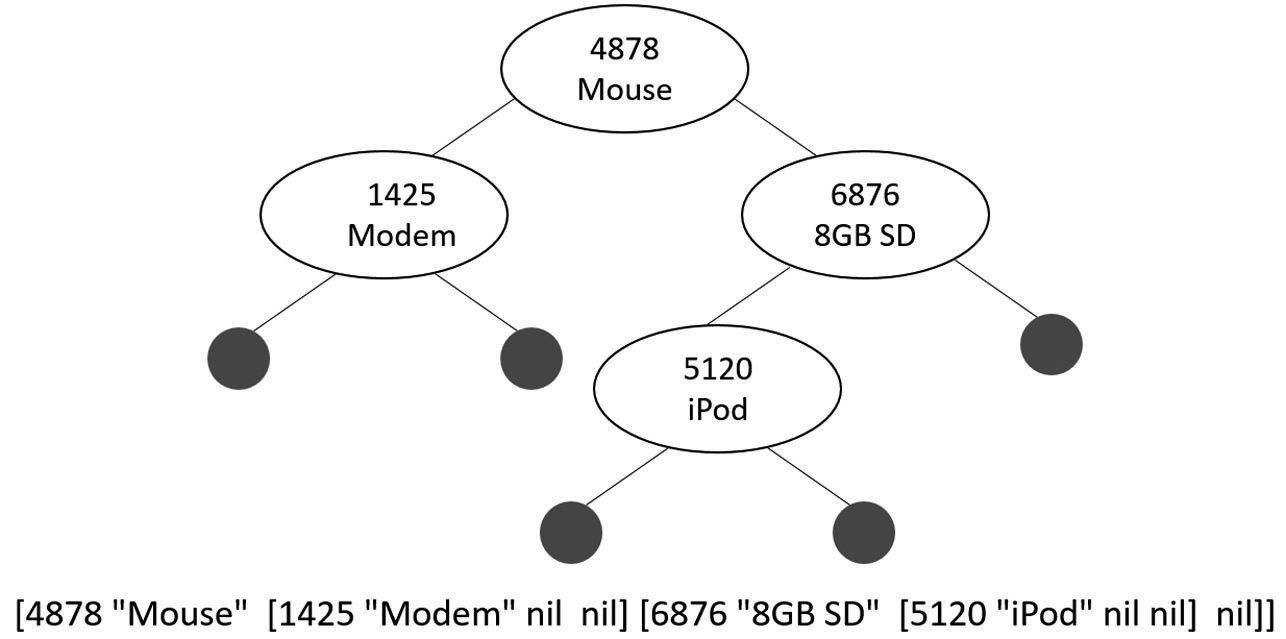
\includegraphics[scale=1]{images-cmyk/searchtree}
\end{center}
\index{tree!diagram}\index{search tree!diagram}\index{AVL tree!diagram}
\index{diagram!AVL tree}
\caption{Search Tree Diagram and Corresponding Formula}
\label{fig:searchtree-diagram}
\end{figure}

\label{height-def}
\index{height!tree}\index{tree!height}
\index{AVL tree!height operator}\index{search tree!height}
The \emph{height} of an empty tree is zero.
The height of a non-empty tree is one more than that of the
taller of its left and right subtrees.
The size of a search tree is the number of keys that occur in the tree,
which is zero for an empty tree, and
for a non-empty tree, is one more than the sum
of the sizes of its left and right subtrees.

We use ACL2 to formalize these definitions
(Figure \ref{fig:tree-functions}, page \pageref{fig:tree-functions}),
starting with an operator \textsf{mktr} to build a tree from its four components.
Then we define operators to extract keys, data, and subtrees from nodes
(\textsf{key}, \textsf{dat}, \textsf{lft}, and \textsf{rgt}).
Finally, we define predicates to recognize keys and search trees
(\textsf{iskeyp}, \textsf{treep}, \textsf{emptyp}),
and to find out whether a key occurs in a tree (\textsf{keyp}).

\begin{figure}
\begin{center}
\begin{code}
\begin{verbatim}
(defun mktr (k d lf rt)            ; make tree from
   (list k d lf rt))               ;  key, data, subtrees
(defun key (s) (first s))          ; key at root
(defun dat (s) (second s))         ; data at root
(defun lft (s) (third s))          ; left subtree
(defun rgt (s) (fourth s))         ; right subtree
(defun emptyp (s) (not (consp s))) ; empty tree?
(defun height (s)                  ; tree height
  (if (emptyp s)
      0                                               ; {ht0}
      (+ 1 (max (height (lft s)) (height (rgt s)))))) ; {ht1}
(defun size (s)                    ; number of keys
  (if (emptyp s)
      0                                     ; {sz0}
      (+ 1 (size (lft s)) (size (rgt s))))) ; {sz1}
(defun iskeyp (k)
   (natp k))
(defun treep (s)                  ; search tree?
  (or (emptyp s)
      (and (= (len s) 4) (natp (key s))
           (treep (lft s)) (treep (rgt s)))))
(defun keyp (k s)                ; key k occurs in s?
  (and (iskeyp k) (treep s) (not (emptyp s))
       (or (= k (key s)) (keyp k (lft s)) (keyp k (rgt s)))))
\end{verbatim}
\end{code}
\end{center}
\index{equation, by name!\{ht0\}, \{ht1\}}
\index{equation, by name!\{sz0\}, \{sz1\}}
\index{height!tree}\index{tree!height}\index{search tree!height}
\index{operator, by name!height (AVL tree)}\seeonlyindex{height (AVL)}{operator}
\index{AVL tree!height operator}
\index{AVL tree!subtree, extract}
\index{AVL tree!representation, formal}\index{search tree!representation}
\index{tree!representation}\index{representation!AVL tree}
\index{operator, by name!mktr (AVL, make tree)}\seeonlyindex{mktr (AVL)}{operator}
\index{AVL tree!mktr operator}
\index{operator, by name!key (AVL, root key)}\seeonlyindex{key (AVL)}{operator}
\index{AVL tree!key operator}
\index{operator, by name!dat (AVL, root data)}\seeonlyindex{dat (AVL)}{operator}
\index{AVL tree!dat operator}
\index{operator, by name!lft (AVL, left subtree)}\seeonlyindex{lft (AVL)}{operator}
\index{AVL tree!lft operator}
\index{operator, by name!size (AVL tree)}\seeonlyindex{size (AVL)}{operator}
\index{AVL tree!size operator}
\index{operator, by name!rgt (AVL, right subtree)}\seeonlyindex{rgt (AVL)}{operator}
\index{AVL tree!rgt operator}
\index{operator, by name!emptyp (AVL, \emph{see} predicate)}
\seeonlyindex{emptyp (AVL)}{predicate}
\index{predicate, by name!emptyp (AVL tree)}
\index{operator, by name!iskeyp (AVL, \emph{see} predicate)}
\seeonlyindex{iskeyp (AVL)}{predicate}
\index{predicate, by name!iskeyp (AVL tree)}
\index{AVL tree!iskeyp predicate}
\index{operator, by name!keyp (AVL, \emph{see} predicate)}
\seeonlyindex{keyp (AVL)}{predicate}
\index{predicate, by name!keyp (AVL, occurs in)}
\index{AVL tree!keyp predicate}
\index{occurs in search tree!keyp (\emph{see} predicate)}
\index{operator, by name!treep (AVL, \emph{see} predicate)}
\seeonlyindex{treep (AVL)}{predicate}
\index{predicate, by name!treep (AVL)}
\index{AVL tree!treep predicate}
\seeonlyindex{treep (AVL)}{predicate}
\caption{Search Tree Operators and Predicates}
\label{fig:tree-functions}
\end{figure}

The only tree of height zero is the empty tree because
the height of a non-empty tree is one more than the maximum
of two other numbers, which makes it at least one.
Theorem \{\emph{ht-emp}\} states this fact more rigorously.

\label{thm:ht-emp}
Theorem \{\emph{ht-emp}\} \textsf{(treep $s$)} $\rightarrow$ ((\textsf{(height $s$) = 0)} $=$ \textsf{(emptyp $s$)})
\section{Ordered Search Trees}

Since keys are natural numbers,
search trees are ordered (page \pageref{ordered-def}) if, for each node,
its key is greater than all of the keys that occur in the left subtree
and less than all the keys that occur in the right subtree.
A empty tree is ordered by default.
The following equations define
the predicate \textsf{ordp} so that
\textsf{(ordp $s$)} is true if $s$ is ordered and false otherwise.

\begin{center}
\label{def:ordp}
\index{predicate, by name!ordp (AVL tree)}\index{AVL tree!ordp predicate}
\seeonlyindex{ordp (AVL tree)}{predicate}
\index{order!AVL tree}\index{AVL tree!order}\index{search tree!order}
\index{equation, by name!\{ord\}}\index{axiom, by name!\{ord\}}
\begin{tabular}{lll}
\textsf{(ordp $s$)} $=$ & \textsf{(emptyp $s$)} $\vee$ & \{\emph{ord}\} \\
             & (\textsf{(treep $s$)}  $\wedge$                        \\
             & ~~($\forall x$.(\textsf{(keyp $x$ (lft $s$)}) $\rightarrow$ $x$ $<$ \textsf{(key $s$)})) $\wedge$ \textsf{(ordp (lft $s$))} $\wedge$ & \\
             & ~~($\forall y$.(\textsf{(keyp $y$ (rgt $s$))} $\rightarrow$ $y$ $>$ \textsf{(key $s$)})) $\wedge$ \textsf{(ordp (rgt $s$))})         & \\
\end{tabular}
\end{center}

Duplicate keys do not occur in ordered search trees.
A more rigorous statement of this fact can be based on
the following observations.\index{duplicate key, none (AVL)}\index{key!duplicates, none}
%\begin{quote}
\begin{enumerate}
\item A key at a node does not occur in either of its subtrees.
\item Any key in one subtree of a node is not equal to the key of the node
      and does not occur in the other subtree.
\end{enumerate}
%\end{quote}
\label{thm:keys-unique}\index{theorem, by name!\{keys unique\}}\index{AVL tree!unique keys theorem}\index{key!unique (theorem)}
%\begin{quote}
Theorem \{\emph{keys unique}\}. \\
$($\textsf{(iskeyp $k$)} $\wedge$ \textsf{(ordp $s$)}$) \rightarrow$ \\
$(((k$ $=$ \textsf{(key $s$)}$) \rightarrow ((\neg$\textsf{(keyp $k$ (lft $s$))}$) \wedge (\neg$\textsf{(keyp $k$ (rgt $s$))}$)))$ $\wedge$ \\
\hspace*{1.5mm}$(($\textsf{(keyp $k$ (lft $s$))}$) \rightarrow ((k$ $\ne$ \textsf{(key $s$)}$) \wedge (\neg$\textsf{(keyp $k$ (rgt $s$)}))$))$ $\wedge$ \\
\hspace*{1.5mm}$(($\textsf{(keyp $k$ (rgt $s$))}$) \rightarrow ((k$ $\ne$ \textsf{(key $s$)}$) \wedge (\neg$(\textsf{keyp $k$ (lft $s$))}$))))$ \\
%\end{quote}

Stating this theorem is more complicated than proving it.
By equation \{\emph{ord}\}, if \textsf{(keyp $x$ (lft $s$))}, then $x$ $<$ \textsf{(key $s$)}.
Since $k$ $=$ \textsf{(key $s$)}, we conclude that $x \neq k$.
That is, ($k$ $=$ \textsf{(key $s$)}$) \rightarrow (\neg$\textsf{(keyp $k$ (lft $s$))}$)$.
That proves one of the implications in the theorem.
The others are as easily dispatched by citing parts
of the definition of the predicate \textsf{ordp}.

\begin{exercises}
\exer {Prove:
\textsf{(ordp $s$)} $\rightarrow ($\textsf{(keyp $k$ (lft $s$))} $\rightarrow$ (($k$ $\ne$\textsf{(key $s$)}) $\wedge (\neg$ \textsf{(keyp $k$ (rgt $s$))}$)))$}

\exer {Prove:
\textsf{(ordp $s$)} $\rightarrow ($\textsf{(keyp $k$ (rgt $s$))} $\rightarrow$ (($k$ $\ne$\textsf{(key $s$)}) $\wedge (\neg$ \textsf{(keyp $k$ (lft $s$))}$)))$}
\end{exercises}

\section{Balanced Search Trees}

Search trees must be ordered to make it convenient to find things.
However, order is not enough.
Trees must also be short, relative to the number of items in the tree.
Otherwise, order doesn't help. %'
It can take as long, on the average, to find an item
in an ordered but unbalanced tree as it would
if the data were completely unorganized.
Figure \ref{fig:unbalanced-trees} (page \pageref{fig:unbalanced-trees})
compares some extremes.

\begin{figure}
\begin{center}
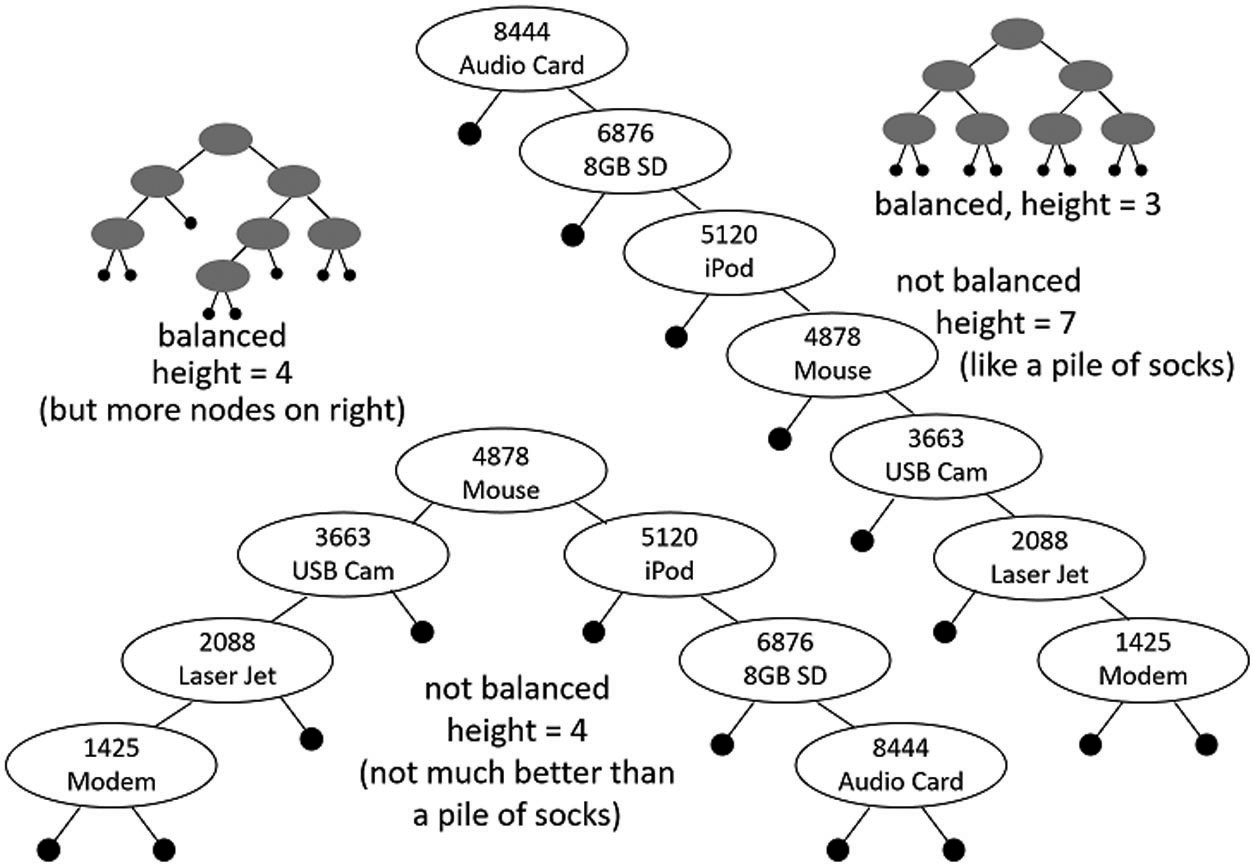
\includegraphics[scale=1]{images-cmyk/unbalanced-trees}
\end{center}
\index{balance!AVL tree}\index{AVL tree!balance}\index{search tree!balance}
\index{AVL tree!unbalanced}
\caption{Balance Shortens Trees}
\label{fig:unbalanced-trees}
\end{figure}

The tree of height seven in
Figure \ref{fig:unbalanced-trees}
is unbalanced at every level.
A binary search on this tree would have no advantage over
looking through a pile of socks, one by one.
The unbalanced tree of height four in the figure is not much better.
It has the same number of nodes in the left subtree as in the right subtree,
but all of the subtrees are maximally unbalanced, like a pile of socks.

Balance is what prevents time-consuming searches, and the unbalanced
examples in Figure \ref{fig:unbalanced-trees} show how bad it can get.
A search tree that, in every node, has two subtrees of the same size
is balanced in terms of both size and height. The tree of height three
in Figure \ref{fig:unbalanced-trees} (page \pageref{fig:unbalanced-trees})
has this maximally balanced shape.
However, the number of steps
required to find a key in a search tree is determined by the heights of subtrees,
not the number of nodes they contain, and
a tree can be balanced with respect to height even though some nodes contain
more keys in one subtree than the other.
The balanced tree of height four in the figure shows how this can happen.
The shape of this tree isn't symmetric at any level,
but no node has subtrees whose heights differ by more than one,
and that's good enough.
We are trying keep the height of a tree with $n$ nodes
within a fixed percentage of $log_2(n)$,
and height balancing is sufficient to accomplish this goal.
\index{balance!AVL tree}\index{AVL tree!balance}\index{search tree!balance}
Full symmetry isn't necessary. %'

As we mentioned before (page \pageref{50pct-thm})
the height of a balanced search tree
turns out to be less than $\frac{3}{2} log_2(n)$.
That makes finding things take more
steps than the optimal case in which both subtrees of
each node contains the same number keys,
but the search still goes fast.
Finding a particular key among a billion nodes
might require 45 steps instead of 30, but that's %'
still plenty fast compared with half a billion steps,
on the average, for unorganized data.

What we get for a few extra steps in finding things is
an astonishing improvement in the number of steps required
to insert a new key or delete an old key.
Instead of $n/2$ steps, on the average,
when keys beyond the point of insertion
all need to be moved to make space for the new one,
insertion can be done in logarithmic time.
That is, the number of steps required to insert
a node in a search tree will be proportional to $log_2(n)$,
giving us the same advantage in insertion speed
that binary search provides in look-up speed.
Deletion can be handled in a similar way, and with the same effectiveness.
That is, search, insertion, and deletion can all be done in logarithmic time.

\begin{exercises}
\exer {\index{height!AVL tree}\index{AVL tree!height operator}%
\index{binary tree!height}\index{tree!height}Find a way to put put $2^n - 1$ keys
in a binary search tree of height $n$.}
\end{exercises}

\section{Inserting a New Item in a Search Tree}

To make search, insertion, and deletion efficient,
search trees must be both ordered and balanced.
We regard to balance,
we must make sure that in every node the heights of the left and right subtrees
differ by one or less.
\label{balance-defun}The predicate \textsf{balp} expresses this notion formally
(Figure \ref{fig:balance-defun}, page \pageref{fig:balance-defun}).

\begin{figure}
\begin{center}
\begin{code}
\begin{verbatim}
(defun balp (s) ; tree s is balanced?
  (or (emptyp s)
      (and (<= (abs (- (height (lft s)) (height (rgt s)))) 1)
           (balp (lft s) (balp (rgt s))))))
\end{verbatim}
\end{code}
\end{center}
\index{balance!AVL tree}\index{AVL tree!balance}\index{search tree!balance}\index{predicate, by name!balp (AVL balance)}\seeonlyindex{balp, AVL tree}{predicate}\index{operator, by name!balp (predicate)}
\caption{Balance Predicate}
\label{fig:balance-defun}
\end{figure}

It isn't difficult to maintain order.
You can do this by moving left or right down the tree according
to whether the new key is less than or greater than the key at the node
under consideration.
When you arrive at an empty tree,
insert a node that has the new key
with its associated data
and has empty trees as its left and right subtrees.
The new tree will be properly ordered because
of the way the procedure located a place to
hook the new key on the tree,
but the new tree will not be balanced if
the location of the new key increases the height
of a subtree that was already taller than its sibling.
Figure \ref{fig:hook-defun} (page \pageref{fig:hook-defun}) provides
an inductive definition of this insertion method.
The definition uses a non-inductive formula
to put the new key into an empty tree
and an inductive formula for the non-empty case.\footnote{In
\label{same-key-new-data}
case the \textsf{hook} operator encounters a key that is the same
as the one it is inserting, it delivers a tree with that key, as it should.
However, the data associated with the new key will be the data supplied
as the second operand in the invocation of \textsf{hook}.
The old data is lost.
This provides a way to associate new data with a key.
The definition might have chosen a different alternative,
but this is a viable one for our purposes.}

\begin{figure}
\begin{center}
\begin{code}
\begin{verbatim}
(defun hook (x a s) ; put a new key x with data a into tree s
  (if (empty s)     ; preserve order, but not necessarily balance
      (mktr x a nil nil)
      (let* ((k  (key s)) (d (dat s))
             (lf (lft s)) (rt (rgt s)))
        (if (< x k)
            (mktr k d (hook x a lf) rt)      ; {hook<}
            (if (> x k)
                (mktr k d lf (hook x a rt))  ; {hook>}
                (mktr x a lf rt))))))        ; {hook=}
\end{verbatim}
\end{code}
\end{center}
\index{operator, by name!hook (AVL insert key)}
\seeonlyindex{hook (AVL insertion)}{operator}
\index{AVL tree!hook (insert key)}
\index{equation, by name!\{hook$<$\}, \{hook$>$\}, \{hook$=$\}}
\caption{Insert New Key, Preserving Order, but Not Balance}
\label{fig:hook-defun}
\end{figure}

Inserting a new key in this way
can throw the tree out of balance.
That happens when
placement of the new key increases the height of a subtree that was
already taller than its sibling.
Then the subtree is two units taller than its sibling,
making the tree unbalanced.
In this case, a rearrangement brings it back into balance
without getting keys out of order.

\begin{aside}{aside:insertion-example}{Inserting New Nodes in Small Trees}
The following example starts with a tree containing one item,
then inserts three new items, one at a time.
We use the formula \textsf{(ins $x$ $a$ $s$)} to denote
the tree produced by inserting the key $x$ and associated
data $a$ into the search tree $s$.

The end result is an ordered,
balanced tree containing four items.
It will aid your understanding
of the insertion process if you draw diagrams similar to Figure
\ref{fig:unbalanced-trees} for the trees denoted by the formulas in the example.
Verify, as you go, that each tree is both ordered and balanced.
\begin{center}
\begin{tabbing}
%
\vspace*{-1.5\topsep}
\rule{\textwidth}{0.5pt}
\vspace*{-\topsep}
%
\\
\textsf{(ins} \= \textsf{1125 "Modem" }\\
     \> \textsf{{[}8444 "Audio Card" nil nil{]})} \\
     \> $\Downarrow$ \\
\textsf{{[}1125 "Modem" nil {[}8444 "Audio Card" nil nil{]}{]}} \\
%
\vspace*{-1.5\topsep}
\rule{\textwidth}{0.5pt}%
\vspace*{-\topsep}
%
\\
\textsf{(ins} \= \textsf{4878 "Mouse"} \\
     \> \textsf{{[}1125 "Modem" nil {[}8444 "Audio Card" nil nil{]}{]})} \\
     \> $\Downarrow$ \\
\textsf{{[}4878 "Mouse"} \= \textsf{{[}1125 "Modem"      nil nil{]}}  \\
              \> \textsf{{[}8444 "Audio Card" nil nil{]}{]}} \\
%
\vspace*{-1.5\topsep}
\rule{\textwidth}{0.5pt}%
\vspace*{-\topsep}
%
\\
\textsf{(ins} \= \textsf{2088 "Laser Jet"} \\
     \> \textsf{{[}4878 "Mouse"} \= \textsf{{[}1125 "Modem" nil nil{]}} \\
     \>               \> \textsf{{[}8444 "Audio Card" nil nil{]}{]})} \\
     \> $\Downarrow$ \\
\textsf{{[}2088 "Laser Jet"} \= \textsf{{[}1125 "Modem" nil nil{]}} \\
                  \> \textsf{{[}4878 "Mouse" nil {[}8444 "Audio Card" nil nil{]}{]}{]}} \\
%
\vspace*{-1.5\topsep}
\rule{\textwidth}{0.5pt}%
\vspace*{-\topsep}
%
\end{tabbing}
\end{center}\index{AVL tree!ins (insert key) examples}
%\caption{Inserting New Nodes in Small Trees}
%\label{aside:insertion-example}
\end{aside}

In small trees, it's easy to find an ad hoc rearrangement that works, %'
as illustrated in Box~\ref{aside:insertion-example}
(page \pageref{aside:insertion-example}),
but we need a procedure that works for all search trees,
not just the small ones where it's easy to see what to do. %'
Figuring out a rearrangement procedure is what the rest
of this chapter is mostly about.

Putting the new node at the bottom may make the tree taller,
but not necessarily.
For example the insertion point might be on the
empty side of a node that has a tree of height one on the other side,
in which case the insertion would leave the height of the tree unchanged.
But, if the height of the tree changes,
how much could it change?
Not by more than one
(Theorem \{\emph{i-ht}\}, Exercise \ref{thm:i-ht}).

If the tree with the new key is taller than the old tree,
the new tree could be unbalanced.
However, because a height of the left subtree of a
balanced tree does not differ from the height of
the right subtree by more than one,
and because the insertion of a new node cannot increase
the height of either subtree by more than one,
the heights of the left and right subtrees in the new tree
cannot differ by more than two.
So, if we can figure out how to rebalance trees where
one subtree is two units taller than its sibling,
we will have found a way preserve balance
while inserting a new node.

\begin{exercises}
\exer {Given any three distinct keys,
there is only one search tree that is ordered, balanced
and contains those three keys but no others.
Explain why.}

\exer {Box~\ref{aside:insertion-example}
(page \pageref{aside:insertion-example}) displays
insertions leading to an ordered, balanced search tree
containing four items.
The resulting trees were chosen from some equally suitable alternatives.
Write formulas for ordered, balanced trees different from
the ones in the example, but still containing the same keys.}

\exer {Prove by induction on tree height
that insertion of a new node does not increase height by more than one.
That is, assuming that $x$ is a key, $s$ is a search tree,
and \textsf{hook} is the operator defined in
Figure \ref{fig:hook-defun} (page \pageref{fig:hook-defun}),
prove the following theorem.
\begin{center}\index{theorem, by name!\{i-ht\}, AVL height after insert}\index{balance!after AVL insert}\index{search tree!balance}\index{tree!balance}\index{height!maximum change in}
\label{thm:i-ht}
Theorem \{\emph{i-ht}\}: $($\textsf{(height $s$)} $=$ $n)$ $\rightarrow$ \textsf{(height (hook $x$ $a$ $s$)) } $\leq n+1$
\end{center}
}

\exer {Use induction on height to prove the following theorem
(\textsf{ordp} is defined on page \pageref{def:ordp}).
\begin{center}\index{theorem, by name!\{i-ord\}, AVL insert}\index{order!AVL insert}
\label{thm:i-ord}
Theorem \{\emph{i-ord}\}
\textsf{(ordp $s$)} $\rightarrow$ \textsf{(ordp (hook $x$ $a$ $s$))}
\end{center}
}

\end{exercises}

\section{Insertion, Case by Case}
Balancing small trees is easy because there are only a few
possibilities to consider. Search trees of height two or less
are always balanced.
\begin{center}
\label{thm:bal-ht2}
\index{theorem, by name!\{bal-ht2\}, AVL height $\le\ 2$}
Theorem \{\emph{bal-ht2}\}. (height $s$) $\leq 2$) $\rightarrow$ (balp $s$).
\end{center}

Working through all the possibilities, one by one,
leads to a proof of this theorem.
A tree of height zero is empty
(Theorem \{\emph{ht-emp}\}, page \pageref{thm:ht-emp}),
and \textsf{(balp nil)} $=$ \textsf{(emptyp nil)} is true, by definition
(Figure \ref{fig:balance-defun}, page \pageref{fig:balance-defun}).
Any tree of height one will consist of a single node,
\textsf{[$k$ $d$ nil nil]}, which is balanced because both subtrees
have the same height (namely, zero).
The formula for a tree of height two must match one of the following templates:
\textsf{[$k$ $d$ [$j$ $c$ nil nil] nil]}, \textsf{[$k$ $d$ nil [$i$ $b$ nil nil]]},
or \textsf{[$k$ $d$ [$j$ $c$ nil nil] [$i$ $b$ nil nil]]}.
Applying the predicate \textsf{balp}
confirms that all of these trees are balanced,
and that completes the proof.

With big trees, there are more possibilities,
but we can reduce part of the problem to
a shorter tree, rely on induction to deal with that tree,
and use the solution produced on the shorter tree
to put together a full solution.
We want to define an insertion operator, \textsf{ins},
to put a new key in
an ordered, balanced search tree,
producing a new search tree that is ordered, balanced,
and contains the new key as well as all of the old ones.
The operator \textsf{hook} (Figure \ref{fig:hook-defun}, page \pageref{fig:hook-defun})
does the job for trees of height zero or one.
The new tree is ordered (Theorem \{\emph{i-ord}\}, page \pageref{thm:i-ord})
and being of height two or less, it is also balanced
(Theorem \{\emph{i-ht}\}, page \pageref{thm:i-ht},
together with Theorem \{\emph{bal-ht2}\}, page \pageref{thm:bal-ht2}).
So, for trees of height zero or one,
the \textsf{hook} operator, by itself, is adequate for
inserting new keys.

That leaves us with trees of height two or more.
We want to define an insertion operator, \textsf{ins},
so that
if $s$ is an ordered, balanced search tree
of height $n+2$ (where $n$ is a natural number),
then the tree \textsf{(ins $x$ $a$ $s$)}
is ordered, balanced, contains all the keys in $s$,
contains the key $x$,
contains no keys other than $x$ and those in $s$,
and has height $n+2$ or $n+3$.
To do this,
we will start with the \textsf{hook} procedure
(which has, already, the order and height properties
that we need for \textsf{ins}),
then find ways to rebalance when it produces
a tree with subtrees whose heights differ by more than one.\footnote{Our
primary concerns will be the issues of height and balance.
The other issues
(presence of the new key, preservation of all the old keys,
etc.)
are easy to work through from the definitions.
An issue that we will gloss over throughout the discussion
is the treatment of data associated with a key.
We include the data in the operator definitions because,
as a practical matter, search trees need some way to
associate data with keys.
Usually, keys just provide a way to find the data.
The operator definitions keep each data item
with its associated key.
Whenever we use \textsf{mktr} to build a tree,
we put the key in the first operand
and the associated data in the second operand.
This keeps the key with its data.
However, that is pretty much the extent of
our analysis of key/data associations.
Doing more is tricky because there are no
constraints on the domain of the data.
The data could even come from a domain
that doesn't support reasoning about equality.
This would be the case, for example, if the data items
were, themselves, operators, and the search tree
were being used to provide organized access to those
operators. There is no algorithm
for determining, in general, whether two operators
denote the same operation,
so it would be difficult to reason about whether or
not key/data associations stay the same throughout the process.}
Our inductive definition of \textsf{ins} will
assume that it has the desired properties
when operating on trees of height less than $n+2$
and prove that, with that assumption, it also
has those properties on trees of height $n+2$.

\begin{figure}
\begin{center}
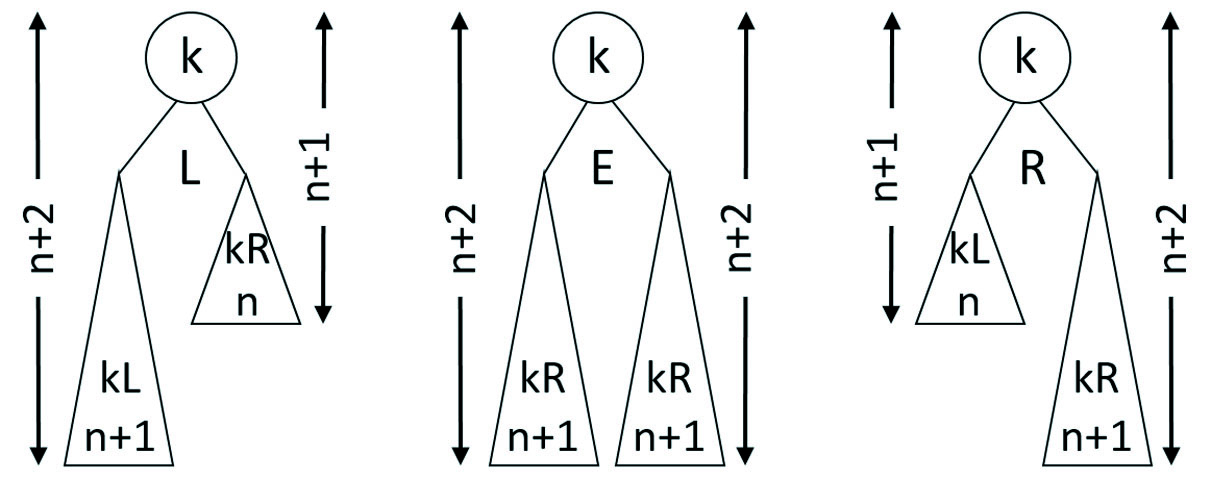
\includegraphics[scale=1]{images-cmyk/ht2-or-more}
\end{center}
\index{tree!balance}\index{search tree!balance}
\index{AVL tree!balance}\index{balance!AVL tree}
\caption{Balanced Trees of Height $n+2$}
\label{fig:trees-of-ht-n+2}
\end{figure}

Diagrams of search trees will help us work through the analysis, case by case.
Figure \ref{fig:trees-of-ht-n+2} (page \pageref{fig:trees-of-ht-n+2})
displays the three configurations that a search tree of height $n+2$ can have.
Each diagram shows the root node as a circle labeled with a name for its key
and shows the left and right subtrees as triangles dangling from the root.
Each triangle represents an ordered, balanced subtree.
A label inside the triangle
simplifies references to the subtree,
and a formula near the bottom of the triangle
specifies the height of the subtree.
Each tree as a whole is labeled with a name near the top of its diagram
(\emph{L}, \emph{E}, and \emph{R}).
The tree \emph{L} is one unit taller on the left than on the right,
\emph{R} is taller on the right, and
both subtrees in \emph{E} have the same height.

An insertion into tree \emph{E} cannot cause the tree to go out of balance
because, at worst, insertion will make one side of the tree
one unit taller than the other side, which leaves the tree
balanced. (The subtrees have height less than $n+2$,
so the induction hypothesis guarantees that they remain
balanced after insertion.)
Therefore, we do not concern ourselves with trees like \emph{E}.
However, if we insert a new key that is less than $k$
into tree \emph{L}, the key would end up in subtree \emph{kL},
the left subtree of \emph{L}, and
the tree could go out of balance
because the height of its left subtree could increase to $n+2$,
while the right subtree would remain at height $n$.
Similarly, inserting a key greater than $k$ into the tree \emph{R}
could make its right subtree \emph{kR} too tall.
Tree \emph{L} and tree \emph{R} represent the cases we need to look into.

\begin{figure}
\begin{center}
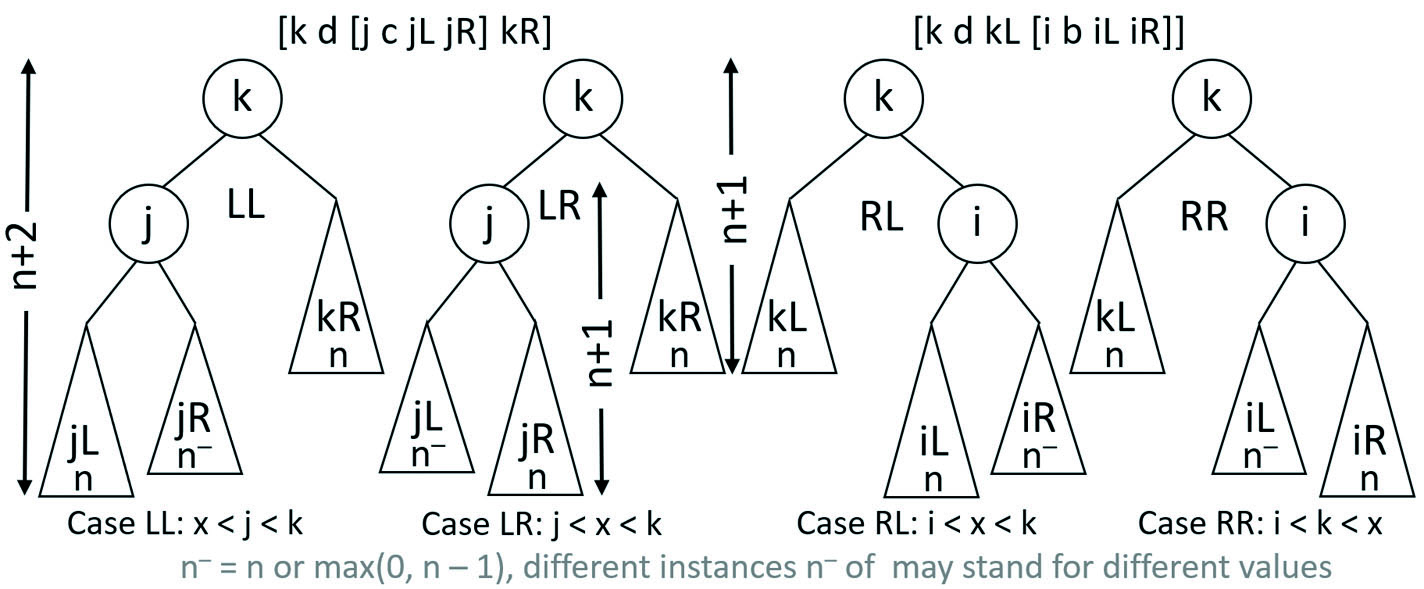
\includegraphics[scale=1]{images-cmyk/ht2-or-more-ex}
\end{center}
\index{tree!balance}\index{search tree!balance}
\index{AVL tree!balance}\index{balance!AVL tree}
\caption{Balanced Trees of Height $n+2$, Subtrees Expanded}
\label{fig:trees-of-ht-n+2-expanded}
\end{figure}

Figure \ref{fig:trees-of-ht-n+2-expanded} (page \pageref{fig:trees-of-ht-n+2-expanded})
will guide deeper analysis.
In the figure, certain subtrees of \emph{L} and \emph{R} from
Figure \ref{fig:trees-of-ht-n+2} (page \pageref{fig:trees-of-ht-n+2})
are expanded to show additional details.
The new diagrams expand subtree
\emph{kL} in tree \emph{L} and subtree \emph{kR} in tree \emph{R}.
Both of these subtrees have height $n+1$.
That makes them non-empty, so each of them must have at least one key.
The expanded diagrams of these subtrees
reveal details about their keys and subtrees.

In tree \emph{L} (Figure \ref{fig:trees-of-ht-n+2}),
the subtree \emph{kL} has height $n+1$,
so at least one of its subtrees has height $n$.
Its sibling might also have height $n$, but (unless $n$ is zero)
it could alternatively have height $n-1$.
The diagrams in Figure \ref{fig:trees-of-ht-n+2-expanded}
and other diagrams in this chapter
use the notation $n^-$
to denote a value that could be either $n$
or, if $n$ isn't zero, $n-1$.
The value denoted by $n^-$ is not necessarily the same
in all of the tree diagrams in the figure,
but the value will be, in every instance,
either $n$ or $n-1$.

Either subtree may be the taller one,
so we draw two diagrams representing the two possibilities
(trees \emph{LL} and \emph{LR}).
Similarly, there are two diagrams for the tree \emph{R},
which makes a total of four tree diagrams in
Figure \ref{fig:trees-of-ht-n+2-expanded}:
two diagrams (\emph{LL} and \emph{LR})
expanding tree \emph{L} from Figure \ref{fig:trees-of-ht-n+2}
and two diagrams (\emph{RL} and \emph{RR}) expanding tree \emph{R}.

Consider the problem of inserting a new key, $x$, into
an ordered, balanced search tree of height $n+2$ with the key $k$
at its root, the key $j$ at the root of its left subtree,
and the key $k$ at the root of its right subtree.
The value of $x$ will fall into one of four intervals.\footnote{We
can ignore the possibility that $x$ is the same as
$k$, $j$, or $i$ because
inserting a key that is the same as one already in the
tree does not change the tree,
except to replace the data associated with the key.
Therefore, the tree will remain balanced and
require no further attention.}\index{tree!balance}\index{search tree!balance}\index{AVL tree!balance}\index{balance!AVL tree}
\label{cases:ht-n+2}\begin{quote}
\begin{enumerate}
\item case \emph{LL}: $x < j < k$
\item case \emph{LR}: $j < x < k$~~~~~~~~~~~\emph{refer to }
\item case \emph{RL}: $k < x < i$~~~~~~~~~~~~~~\emph{Figure \ref{fig:trees-of-ht-n+2-expanded}}
\item case \emph{RR}: $k < i < x$
\end{enumerate}
\end{quote}

The names of the cases correspond
to the tree diagram in
Figure \ref{fig:trees-of-ht-n+2-expanded} (page \pageref{fig:trees-of-ht-n+2-expanded}).
For example, if the new key $x$ is less than $k$,
insertion cannot cause the tree to go out of
balance unless the left subtree is taller
than the right subtree, which focuses the
analysis on trees \emph{LL} and \emph{LR}
in the figure.
We use \emph{LL} for the case when the new key $x$
is smaller than the key $j$
($x < j < k$)
because that pushes the key into subtree \emph{jL},
and the tree \emph{LL} will definitely go out of balance
if insertion increases the height of \emph{jL}.
The analysis of case \emph{LL} covers
subtrees \emph{jR} both of height $(n-1)$ and of height $n$.

\begin{figure}
\begin{center}
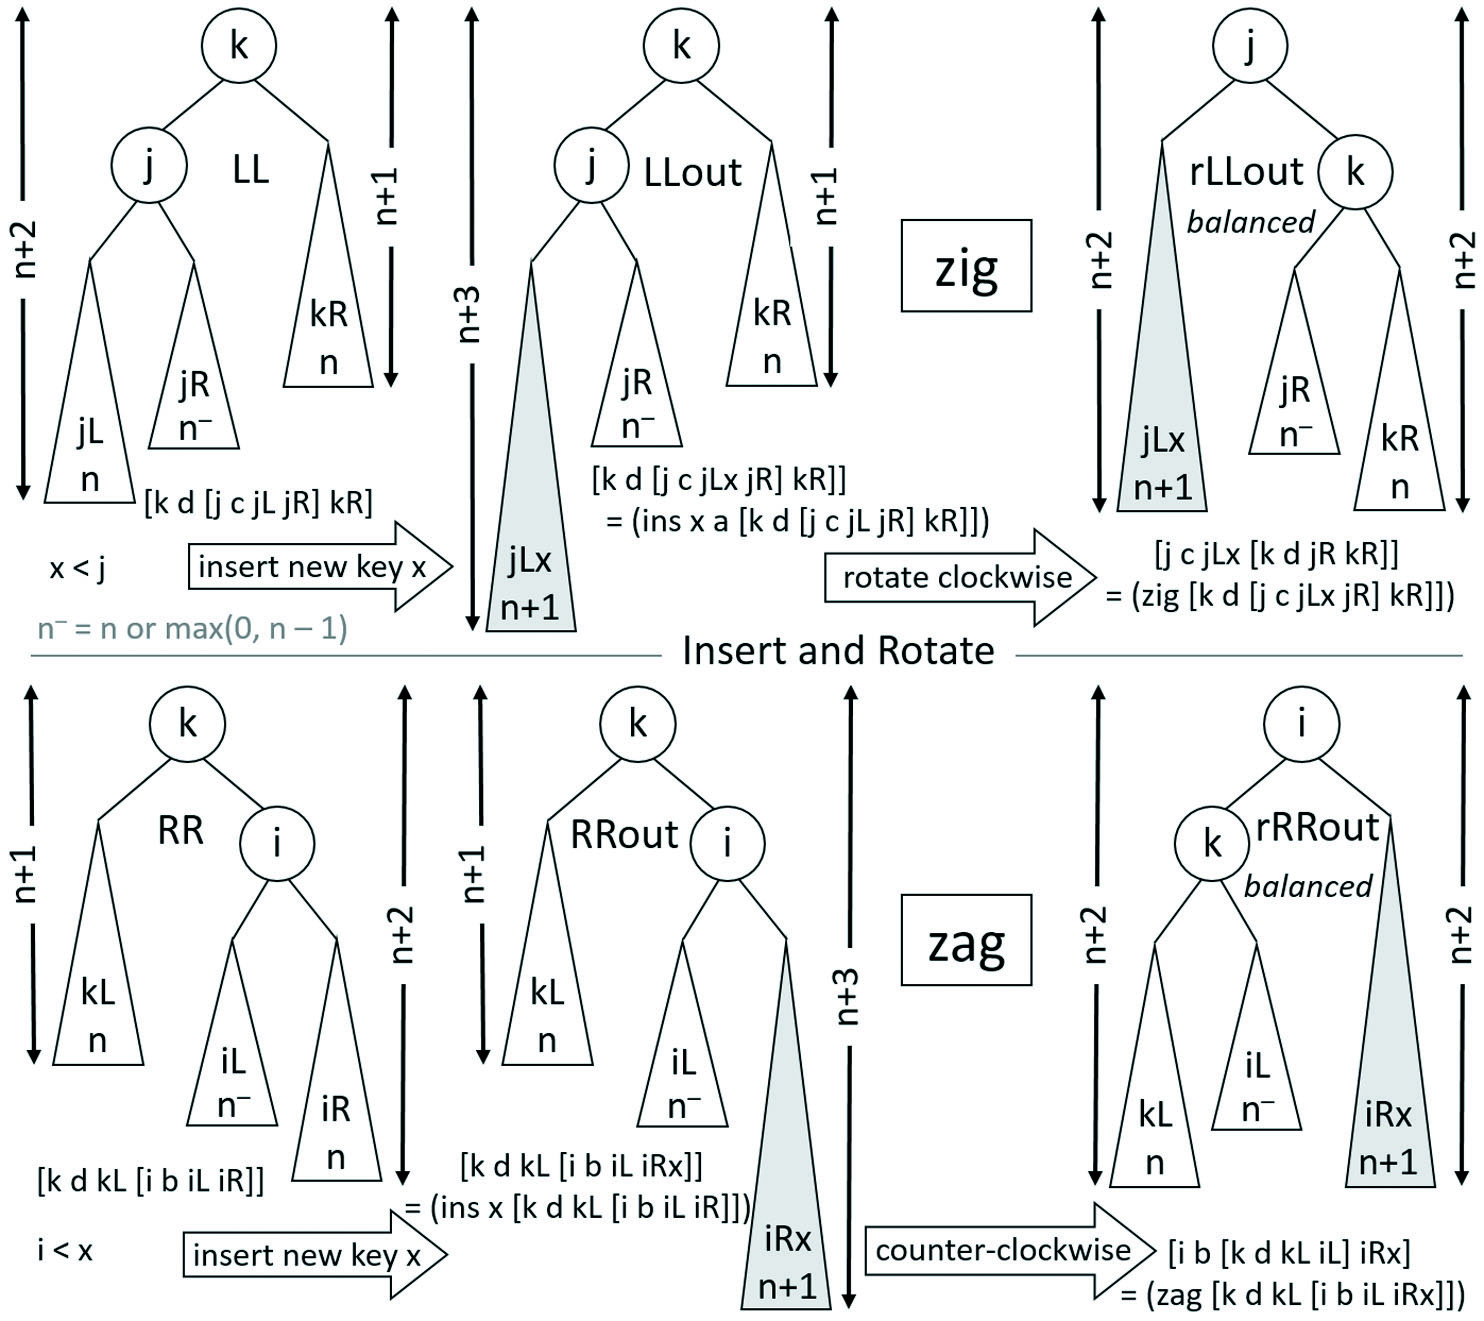
\includegraphics[scale=1]{images-cmyk/zig-and-zag}
\end{center}
\index{tree!rebalance}\index{search tree!rebalance}
\index{AVL tree!rebalance}\index{balance!AVL rebalance}
\caption{Insertion, Unbalanced Outcome, and Rebalancing}
\label{fig:zig-and-zag}
\end{figure}

If the new key $x$ were between $j$ and $k$ ($j < x < k$),
it would go into the subtree \emph{jR}.
That might not cause the tree \emph{LL} to go out of balance,
even if it increases the height of
the subtree \emph{jR}, because in tree \emph{LL}
the subtree \emph{jR} may be shorter than its sibling.
So, we use the diagram of tree \emph{LR}
(where an insertion into subtree \emph{jR}
that increases its height will definitely
produce a tree that is out of balance)
to analyze the insertion of a
key $x$ that lies between $j$ and $k$.
The analysis of case \emph{LR} covers
subtrees \emph{jL} both of height $(n-1)$ and of height $n$.

Case \emph{RR} mirrors
case \emph{LL} and deals with the situation when the new key $x$
is greater than $i$ ($k < i < x$).
Case \emph{RL} mirrors case \emph{LR} and
deals with the situation when the new key $x$
is between $k$ and $i$ ($k < x < i$).
To summarize, we start with $j < k < i$ and
a new key $x$. The new key has to be in one of
four places:
$x < j < k$ (case \emph{LL}),
$j < x < k$ (case \emph{LR}),
$k < x < i$ (case \emph{RL}), or
$k < i < x$ (case \emph{RR}).
The four cases cover all the of the possibilities, so
an analysis of all four cases is a complete analysis
of the insertion procedure.

Case \emph{LL} is the problem of inserting
a key $x$ that is less than $j$
into the tree \emph{LL}.
The new key will go into the subtree \emph{jL}.
Since the height, $n$, of \emph{jL} is less than $n+2$,
the induction hypothesis says that the new subtree,
after insertion,
will be balanced and have height $n$ or $n+1$.
If it has height $n$, the tree, as a whole, remains
balanced, and nothing further needs to be done.
If it has height $n+1$, the tree, as a whole,
will be out of balance (too tall on the left).
It will need rebalancing.

Figure \ref{fig:zig-and-zag} (page \pageref{fig:zig-and-zag})
displays the tree \emph{LL} before insertion
(as it appeared in Figure \ref{fig:trees-of-ht-n+2-expanded})
and a new, unbalanced tree, \emph{LLout}, which represents
the outcome of hooking a new key $x$ ($x < j$) into \emph{LL}.
In the diagram of \emph{LLout}, the subtree
\emph{jLx} is the one with the new key.
The subtree \emph{jLx} has height $n+1$,
which makes \emph{LLout} too tall on the left.
Figure \ref{fig:zig-and-zag} also presents the mirror insertion
into \emph{RR} of a key
$x$ ($i < x$),
producing a tree labeled \emph{RRout}
that is too tall on the right.

Because these insertions lead to unbalanced trees,
we need to rearrange them in some way,
and Figure \ref{fig:zig-and-zag} shows how to do that.
In the case of \emph{LLout},
the key $j$ can go at the root, and the former root key, $k$,
can hang from the right side of the new root.
If we then plug the subtrees into the only places they
can go that preserves order,
the result, tree \emph{rLLout} (Figure \ref{fig:zig-and-zag}),
is balanced and has height $n+2$.
Voila! Like magic.

This clockwise rotation of the tree \emph{LLout},
as shown in the figure,
is traditionally called \textsf{zig}.
The mirror operation, \textsf{zag}, rotates counter-clockwise to fix
the tree \emph{RRout}, which is too tall on the right.
Formal definitions of these rotation operators reside in
Figure \ref{defun:zig-and-zag} (page \pageref{defun:zig-and-zag}).
The definitions emerge in a straightforward way from
the diagrams in Figure~\ref{fig:zig-and-zag}.

\begin{figure}
\begin{center}
\begin{code}
\begin{verbatim}
(defun zig (s) ; rotate clockwise
  (let* ((k  (key s)) (d (dat s))
         (j  (key (lft s))) (c  (dat (lft s)))
         (jL (lft (lft s))) (jR (rgt (lft s)))
         (kR (rgt s)))
    (mktr j c jL (mktr k d jR kR))))
(defun zag (s) ; rotate counter-clockwise
  (let* ((k  (key s)) (d (dat s))
         (kL (lft s))
         (i (key (rgt s))) (b (dat (rgt s)))
         (iL (lft (rgt s))) (iR (rgt (rgt s))))
    (mktr i b (mktr k d kL iL) iR)))
\end{verbatim}
\end{code}
\end{center}
\index{tree!rebalance}\index{search tree!rebalance}
\index{AVL tree!rebalance}\index{balance!AVL rebalance}
\index{operator, by name!zig, zag (AVL rotate)}
\index{AVL tree!zig, zag operators}
\seeonlyindex{zig, zag (AVL rotate)}{operator}
\index{rotate AVL!zig, zag}
\caption{Rotation Operators: \textsf{zig} and \textsf{zag}}
\label{defun:zig-and-zag}
\end{figure}

The rotation trick fixes unbalanced trees that come
from cases \emph{LL} and \emph{RR} (page \pageref{cases:ht-n+2}).
That leaves us with the other two cases:
case \emph{LR} ($j < x < k$) and
case \emph{RL} ($k < x < i$).
We turn our attention to these problems in the next section.

\begin{exercises}
\exer {Prove
\label{thm:unbal-ht3}
Theorem \{\emph{unbal-ht3}\}:
If $s$ is an unbalanced tree of height three,
then one subtree of $s$ is empty and the other has height two.
That is, prove the following implication.
\begin{center}
\begin{tabular}{l}
$(($\textsf{(height $s$)} $= 3) \wedge (\neg$ \textsf{(balp $s$)}$))
\rightarrow$  \\
$(($\textsf{((height (lft $s$))} $= 2) \wedge$ \textsf{(emptyp (rgt $s$))}$)
\vee$
\textsf{((emptyp (lft $s$))} $\wedge ($\textsf{(height (rgt $s$))} $= 2)))$\\
\end{tabular}
\end{center}
}
\end{exercises}

\section{Double Rotations}

Cases \emph{LR} and \emph{RL} (page \pageref{cases:ht-n+2})
are the only two remaining cases that we need to cover to arrive
at a complete solution of the insertion problem.
The cases we already solved
(cases \emph{LL} and \emph{RR})
are known as the
\index{rotate AVL!outside cases}\index{outside cases!AVL rotate}``outside cases''
because the subtrees that
get the new keys and become too tall are on the outside borders of the diagram.
Cases \emph{LR} and \emph{RL}
are \index{rotate AVL!inside cases}\index{inside cases!AVL rotate}``inside cases''
because the problematic subtrees
are on the inside portion of the tree diagram, away from the borders.
Another way to look at it is that $x$ is outside of the interval
between $j$ and $i$ in the outside cases,
and inside the interval in the inside cases.

\begin{center}
\begin{tabular}{llll}
\label{inside-lf} &Inside Left Case \emph{LR}:  &\textsf{(ins $x$ $a$} \emph{LR}\textsf{)}, when $j < x < k$ &
                    \emph{refer to} \\
\label{inside-rt} &Inside Right Case \emph{RL}: &\textsf{(ins $x$ $a$} \emph{RL}\textsf{)}, when $k < x < i$  &~~~\emph{Figure \ref{fig:trees-of-ht-n+2-expanded}, page \pageref{fig:trees-of-ht-n+2-expanded}} \\
\end{tabular}
\end{center}
%\end{comment}
The inside cases are trickier.
Figure \ref{fig:inside-cases} (page \pageref{fig:inside-cases})
shows how insertions into the trees \emph{LR} and \emph{RL}
can make an inside subtree too tall.

\begin{figure}
\begin{center}
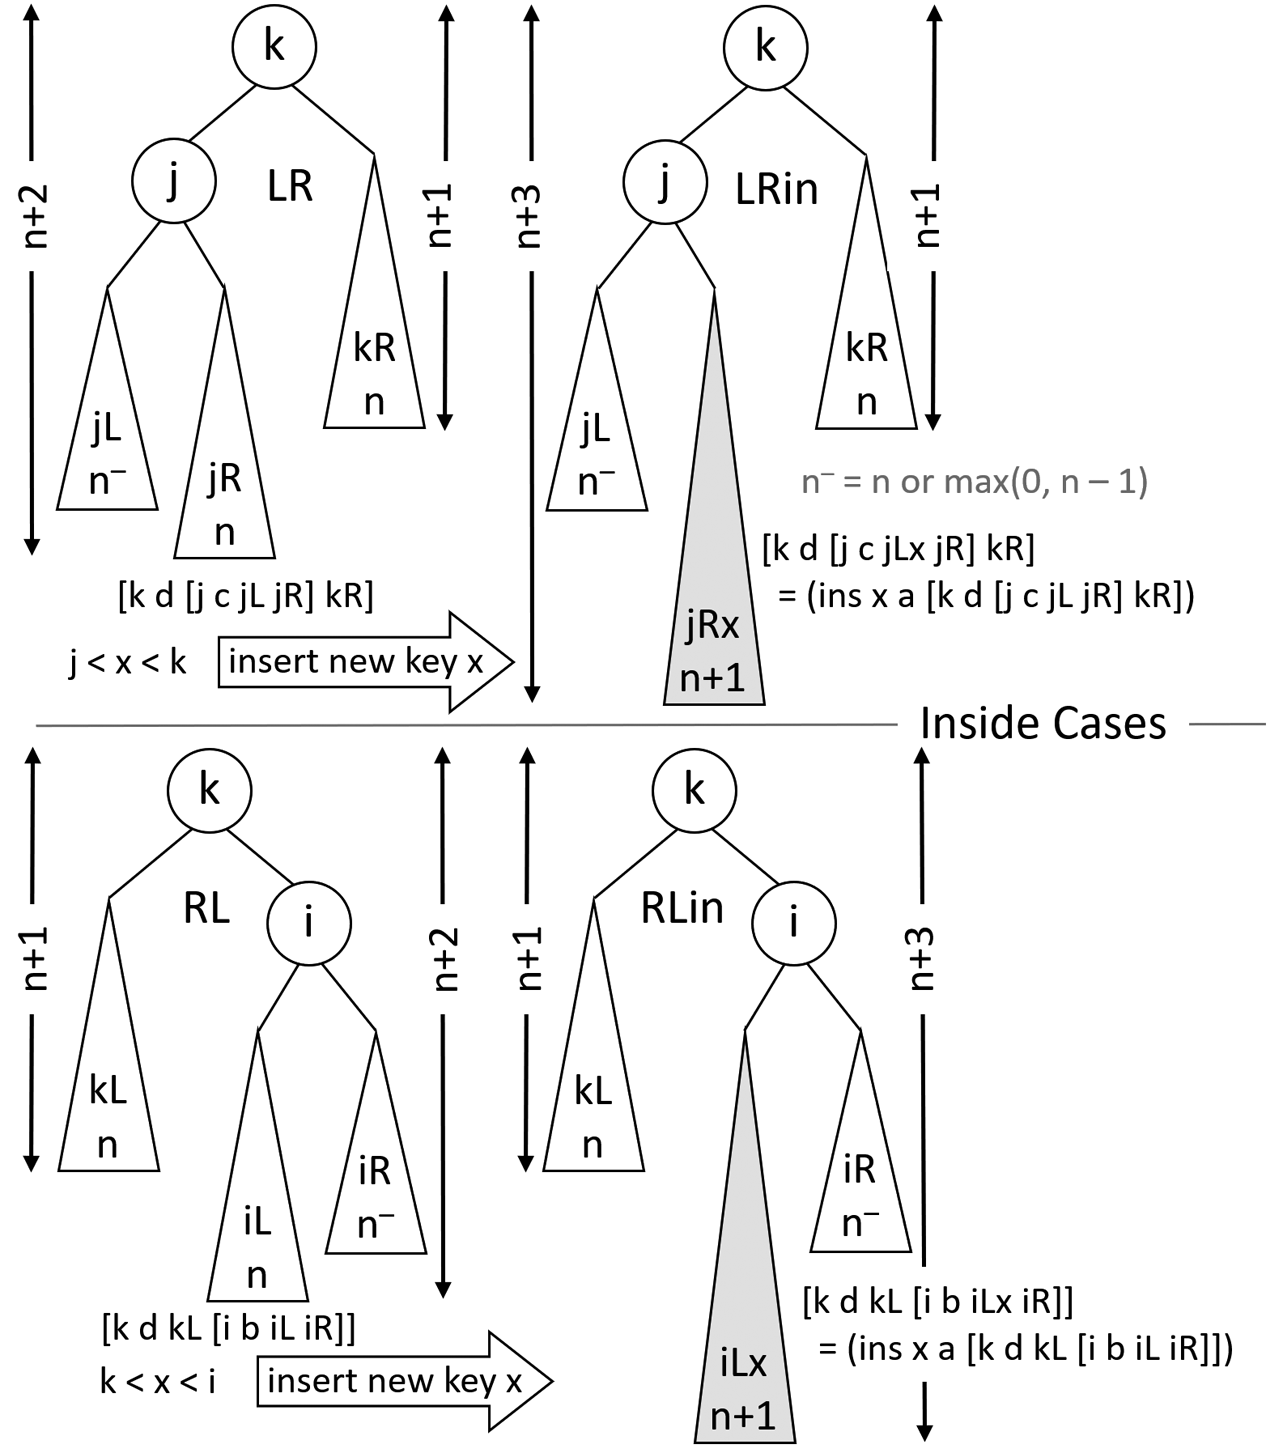
\includegraphics[scale=1]{images-cmyk/inside-cases}
\end{center}
\index{tree!rebalance}\index{search tree!rebalance}
\index{AVL tree!rebalance}\index{balance!AVL rebalance}
\index{rotate AVL!inside cases}\index{inside cases!AVL rotate}
\caption{Inside Cases}
\label{fig:inside-cases}
\end{figure}

Consider tree \emph{LRin} in
Figure \ref{fig:inside-cases}.
A first guess might be that the tree \emph{LRin}
could benefit from a clockwise rotation.
However, that produces a tree with a left subtree of height $n$ or $n+1$
and a right subtree of height $n+3$
(see Figure \ref{fig:badzig}, page \pageref{fig:badzig}).
That is, applying the rotation operator, \textsf{zig}, to \emph{LRin}
leads to a tree that is at least as out of balance as \emph{LRin}.
Clockwise rotation doesn't help.
We need a new trick to rebalance \emph{LRin}.

\begin{figure}
\begin{center}
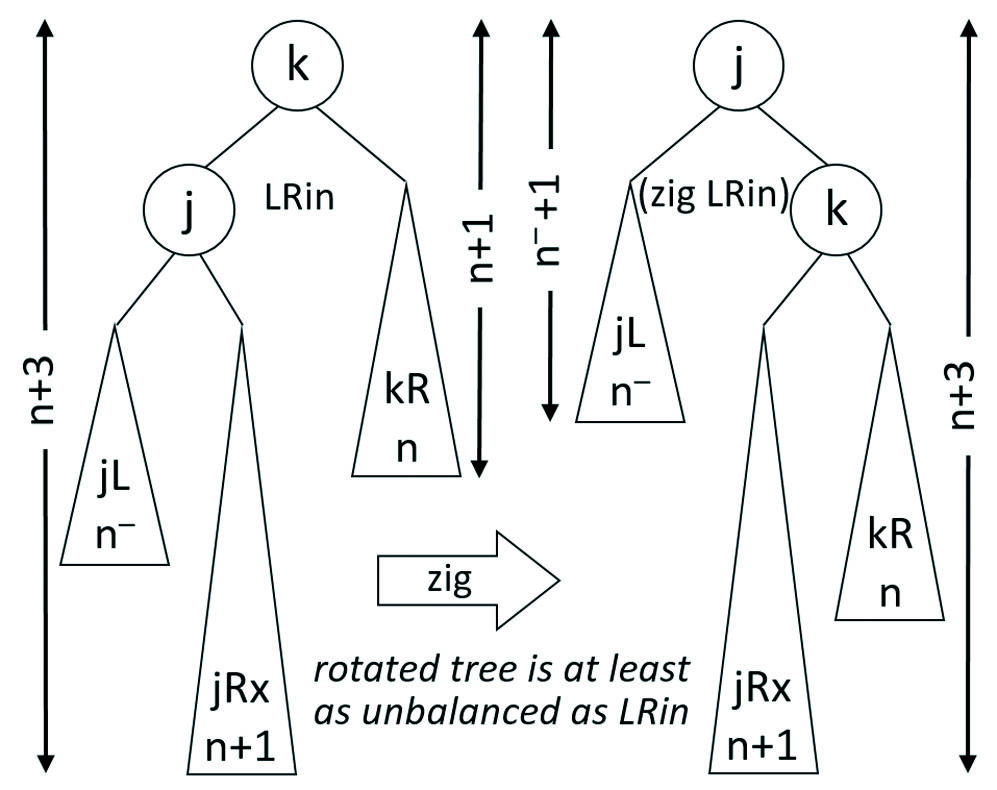
\includegraphics[scale=1]{images-cmyk/badzig}
\end{center}
\index{tree!rebalance}\index{search tree!rebalance}
\index{AVL tree!rebalance}\index{balance!AVL rebalance}
\index{rotate AVL!unbalance}
\caption{Using the Wrong Rotation Can Make It Worse}
\label{fig:badzig}
\end{figure}

The height of subtree \emph{jRx}
(Figure \ref{fig:inside-cases}) is $n+1$,
so at least one of its subtrees has height $n$.
The diagram on the left side of
Figure \ref{fig:dbl-rotation} (page \pageref{fig:dbl-rotation})
shows \emph{jRx} expanded to reveal its key $y$,
left subtree \emph{yL}, shown with height $n^-$,
and right subtree \emph{yR}, shown with height $n$.
The heights of subtrees \emph{yL} and \emph{yR} are either the same,
or \emph{yL} is one unit shorter. It could
have been the other way around, with
\emph{yL} having height $n$ and \emph{yR}, height $n^-$,
but the analysis is the same either way.
We will pursue the alternative
displayed in Figure~\ref{fig:dbl-rotation},
and leave it to you to draw the diagram the other way
and make sure it works. The exercise will be good practice.

\begin{figure}
\begin{center}
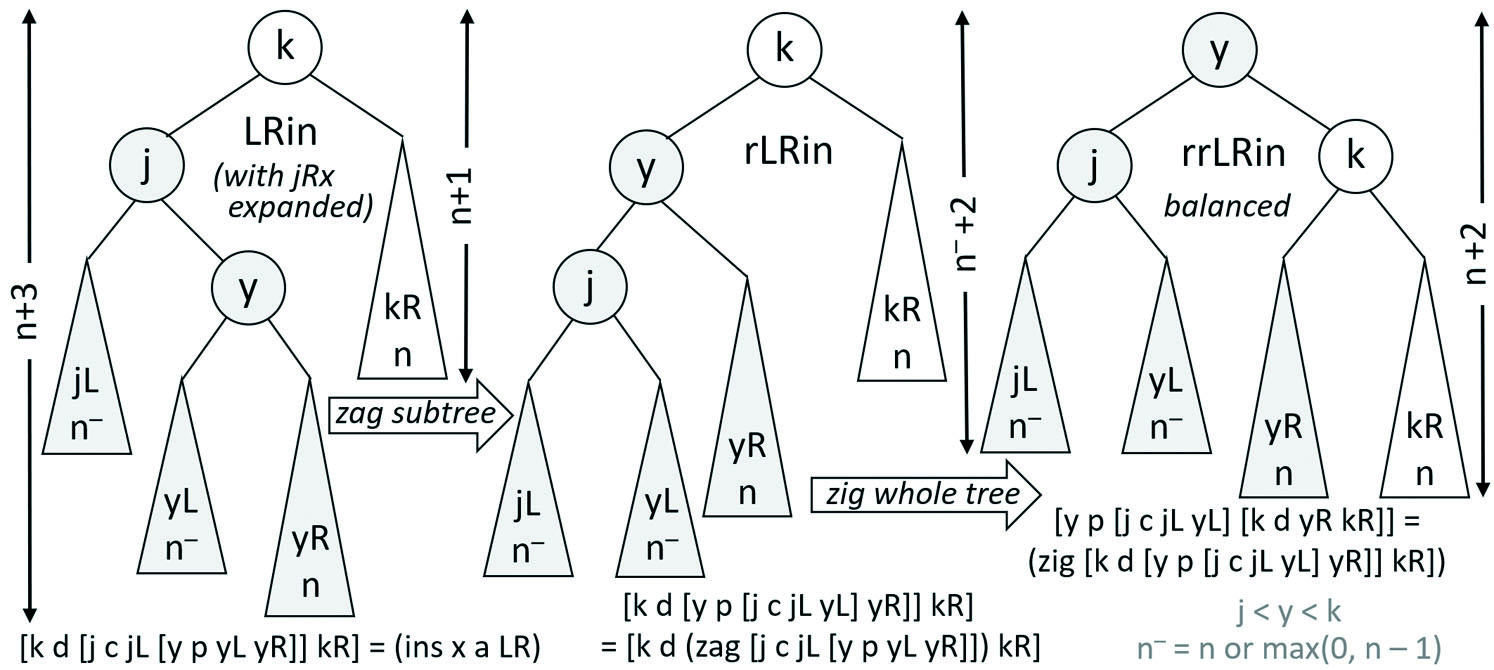
\includegraphics[scale=1]{images-cmyk/dbl-rotation}
\end{center}
\index{tree!rebalance}\index{search tree!rebalance}
\index{AVL tree!rebalance}\index{balance!AVL rebalance}
\index{rotate AVL!inside, double}\index{inside cases!double rotate}
\index{double rotation, AVL}\index{AVL tree!rotate, double}
\caption{Double Rotation Rebalances Inside Cases}
\label{fig:dbl-rotation}
\end{figure}

The diagram in Figure~\ref{fig:dbl-rotation}
makes it clear that we can apply \textsf{zag}
(counterclockwise rotation)
to the left subtree of \emph{LRin}.
It's a counterintuitive move, might not help, might even make things worse,
but it's possible, nonetheless.\footnote{\label{no-zag}It would not be possible
to do a \textsf{zag} rotation if \emph{jRx} were empty.}
The algebraic formula \textsf{[$y$ $p$} \emph{yL} \emph{yR}\textsf{]} in Figure~\ref{fig:dbl-rotation}
is the expansion of subtree \emph{jRx} (Figure~\ref{fig:inside-cases}) to display
its key ($y$) and its subtrees (\emph{yL} and \emph{yR}).
The formula uses $p$ to denote the data associated with key $y$.

After applying the \textsf{zag} operator to the left subtree of tree \emph{LRin}
(Figure~\ref{fig:dbl-rotation}), we the new tree \emph{rLRin} displayed in
the middle of the figure. The left subtree of the new tree \emph{rLRin} has the following algebraic formula.
\begin{center}
\textsf{(zag (lft} \emph{LRin}\textsf{))} =
\textsf{(zag [$j$ $c$} \emph{jL} \textsf{[$y$ $p$} \emph{yL} \emph{yR}\textsf{]])} =
\textsf{[$y$ $p$ [$j$ $c$} \emph{jL} \emph{yL}\textsf{]} \emph{yR}\textsf{]}
\end{center}

To repeat, starting from the unbalanced search tree \emph{LRin}
on the left side of Figure \ref{fig:dbl-rotation},
the middle portion of the figure displays the tree \emph{rLRin},
which is \emph{LRin} with \textsf{zag} applied to its left subtree.
The tree \emph{rLRin}
is not balanced, but the subtree that is too tall
(namely, \textsf{[$y$ $p$ [$j$ $c$} \emph{jL} \emph{yL}\textsf{]} \emph{yR}\textsf{]})
is on the outside left part of \emph{rLRin}.
Therefore, we can apply \textsf{zig} to \emph{rLRin}, as a whole,
to get it back in balance.
\begin{center}
\textsf{(zig} \emph{rLRin}\textsf{)} $=$
\textsf{(zig [$k$ $d$ [$y$ $p$ [$j$ $c$} \emph{jL} \emph{yL}\textsf{]} \emph{yR}\textsf{]]} \emph{kR}\textsf{])} $=$
\textsf{[$y$ $p$ [$j$ $c$} \emph{jL} \emph{yL}\textsf{] [$k$ $d$} \emph{yR} \emph{kR}\textsf{]]}
$=$ \emph{rrLRin}
\end{center}
This second rotation leads to
the tree \emph{rrLRin},
diagrammed on right-hand side of
Figure \ref{fig:dbl-rotation},
which is balanced and has height $n+2$.
Hallelujah! Wonders never cease.

Figure \ref{defun:rot+} (page \pageref{defun:rot+})
formalizes the rebalancing of trees
that have become too tall on the left, due to the
insertion of a key that is less than the key at the root.
The operator \textsf{rot}+, which is defined in the figure,
chooses whether to apply a single rotation,
double rotation, or no rotation
(depending on subtree heights)
and uses the \textsf{zig} and \textsf{zag} operators
(Figure \ref{defun:zig-and-zag}, page \pageref{defun:zig-and-zag})
to carry the necessary rotations, if there are any.

\begin{figure}
\begin{center}
\begin{code}
\begin{verbatim}
(defun rot+ (s)            ; rotate clockwise if too tall on left
  (let* ((k  (key s)) (d  (dat s))  ; rot+ assumes s is not empty
         (kL (lft s)) (kR (rgt s)))
    (if (> (height kL) (+ (height kR) 1))           ; unbalanced?
        (if (< (height (lft kL)) (height (rgt kL))) ; inside lft?
            (zig(mktr k d (zag kL) kR))             ; dbl rotate
            (zig s))                                ; sngl rotate
        s)))                                        ; no rotate
\end{verbatim}
\end{code}
\end{center}
\index{tree!rebalance}\index{search tree!rebalance}
\index{AVL tree!rebalance}\index{balance!AVL rebalance}
\index{rotate AVL!formal}\index{AVL tree!rotate}
\index{double rotation, AVL}
\index{operator, by name!rot+ (AVL rotate)}
\caption{Formal Definition of the Clockwise Rotation Operator}
\label{defun:rot+}
\end{figure}

The operator \textsf{rot}+ performs a clockwise
rotation on a tree that is too tall on the left
(that is, a tree with a left subtree whose height exceeds that
of its right subtree by two).
Assuming that, before rotation,
the tree is ordered and that all of its subtrees are balanced,
the tree that \textsf{rot}+ delivers will be ordered and balanced,
as our case-by-case analysis showed.
If \textsf{rot}+ is applied to a tree whose left subtree
is the same height as its right subtree,
or possibly one unit taller, \textsf{rot}+ delivers its operand as-is,
because it is already a balanced tree.
Likewise, \textsf{rot}+ delivers its operand, as-is,
if the left subtree is shorter than the right subtree.
Counter-clockwise rotation is the mirror image of \textsf{rot}+.
We will use the name \textsf{rot-} for the counter-clockwise rotation operator
and leave its definition as an exercise.

There are no other cases in which insertion
can cause the tree to go out of balance,
so the proof by induction of the
order, balance, and height properties
of the insertion operator, \textsf{ins}, is complete, and
Figure \ref{defun:ins} (page \pageref{defun:ins})
displays the formal definition of \textsf{ins}.

The definition is inductive.
The new key goes into the left subtree
if it is smaller than the key at the root,
and into the right subtree if it is greater.
If the new key is the same as the one at the root,
the insertion operator puts new the data at the root
with that key.\footnote{This treatment
of the key/data association is
as with the \textsf{hook} operator and for the same reasons
(page \pageref{same-key-new-data}).}
If the insertion produces, at first, an unbalanced tree,
it is rebalanced by \textsf{rot}+ or \textsf{rot-}.

\begin{figure}
\begin{center}
\begin{code}
\begin{verbatim}
(defun ins (x a s)
  (if (emptyp s)
      (mktr x a nil nil)                          ; one-node tree
      (let* ((k  (key s)) (d  (dat s))
             (kL (lft s)) (kR (rgt s)))
        (if (< k x)
            (rot+ (mktr k d (ins x a kL) kR))     ; insert left
            (if (> k x)
                (rot- (mktr k d kL (ins x a kR))) ; insert right
                (mktr x a kL kR))))))             ; new root data
\end{verbatim}
\end{code}
\end{center}
\index{operator, by name!ins (AVL insert key)}
\seeonlyindex{ins (AVL insert)}{operator}
\index{AVL tree!ins (insert key) operator}
\caption{Formal Definition of the Insertion Operator}
\label{defun:ins}
\end{figure}

To make search trees really useful, we need to be able to delete items
as well as insert them.
Deletion is a little more complicated than
insertion, but uses the same basic rotation operators.
You know enough, now, to explore the AVL deletion operator on your own.
You can check it out online or a in textbook on algorithms.

\begin{exercises}
\exer {A footnote on page \pageref{no-zag} points out
that is it not possible to apply the \textsf{zag} operator to
a tree whose right subtree is empty.
Similarly, \textsf{zig} does not apply to a tree whose left subtree is empty.
Explain why.}

\exer {Prove that \textsf{(ins $x$ $a$ nil)} delivers a tree that is
ordered and balanced.}

\exer {Prove that \textsf{(ins $x$ $a$ $s$)}
delivers an ordered, balanced tree if (height $s$) = 1.}

\exer {Define \textsf{rot-} \label{defun:rot-}
(see the definition of \textsf{rot}+, page \pageref{defun:rot+}).}

\end{exercises}

\section{Fast Insertion}

The rotation operators, \textsf{rot}+ and \textsf{rot-}, as discussed so far,
compute the heights of the subtrees to choose the proper rotation.
This takes a lot of time because it requires
looking through all the ways to get from the root to the leaves.\footnote{A
leaf is a search tree whose left and right subtrees are both empty.}
To do this, all of the nodes must be examined, so the number of steps in
the computation is proportional to the number of nodes in the tree.
Furthermore, since \textsf{ins} has to check
for possible rotations at every level in the
tree, there are a great many height computations to perform, and this
makes the insertion process take way too many computation steps.

\begin{figure}
\begin{center}
\begin{code}
\begin{verbatim}
(defun ht (s) ; extract height of tree s
  (if (empty s)
      0
      (fifth s)))
(defun mktr (k d lf rt) ; make tree from key, data, and subtrees
    (list k d lf rt h (+ 1 (max (ht lf) (ht rt)))))
(defun treep (s) ; search tree?
  (or (emptyp s)
      (and (n-element-list 5 s) (iskeyp (key s))
           (treep (lft s)) (treep (rgt s))
           (= (ht s) (+ 1 (max (ht(lft s)) (ht(rgt s))))))))
(defun rot+ (s) ; rotate clockwise if too tall on left
  (let* ((k  (key s)) (d  (dat s)) ; rot+ assumes s is not empty
         (kL (lft s)) (kR (rgt s)))
    (if (> (ht kL) (+ (ht kR) 1))           ; unbalanced?
        (if (< (ht (lft kL)) (ht (rgt kL))) ; inside lft?
            (zig(mktr k d (zag kL) kR))     ; dbl rotate
            (zig s))                        ; sngl rotate
        s)))                                ; no rotate
\end{verbatim}
\end{code}
\end{center}
\index{operator, by name!ht (AVL height, fast)}
\index{operator, by name!mktr, fast}
\index{AVL tree!ht (height, fast)}
\index{AVL tree!mktr, fast}
\index{AVL tree!treep predicate, fast}
\index{predicate, by name!treep, fast (AVL)}
\index{operator, by name!treep (AVL, \emph{see} predicate)!fast (\emph{see} predicate)}
\seeonlyindex{ht (AVL height, fast)}{operator}
\index{operator, by name!rot+ (AVL rotate)!fast}
\seeonlyindex{rot+}{operator}
\index{AVL tree!rotate, fast}
\index{rotate AVL!fast}
\caption{Revised Operators To Avoid Height Computation}
\label{defun:balance-factor}
\end{figure}

Fortunately, there is a way to avoid the
\index{operator, by name!ht (AVL height, fast)}
\index{AVL tree!ht (height, fast)}height computation
by recording tree height
in each node along with keys, data, and subtrees.
When a new tree is formed from a key, data, and two subtrees,
its height can be recorded quickly by extracting the heights of the
subtrees, adding one to the larger of those heights,
and recording the result with the key, data, and subtrees.
We use the term ``extracting'' instead of ``computing''
because the height of a subtree is right there with the key.
Extracting the height is a non-inductive operation,
just like extracting the key.\footnote{The situation
is even better than it seems because
it's not the height that the rotation operators need to know.
It's the difference between the heights of the subtrees,
which is known as the \index{AVL tree!balance factor}\index{balance factor (AVL)}\emph{balance factor}.
Because AVL trees are balanced,
the balance factor will always be
-1, zero, or +1.
Keeping track of balance factors is no more difficult
than keeping track of heights,
and balance factors are a little more
efficient in terms of time and space.
However, going this route would require several
more changes in the formal definitions,
so we'll just stick with heights to avoid complicating the presentation.}

To use the approach that avoids
the time-consuming computation of height,
a few of the operators implementing the AVL solution
(Figure~\ref{fig:tree-functions}, page \pageref{fig:tree-functions}, and
Figure~\ref{defun:rot+}, page \pageref{defun:rot+})
must change.

%\begin{quote}
\begin{enumerate}
\item The \textsf{mktr} operator must put the height in the tree it builds.
\item The new height operator, \textsf{ht},\index{operator, by name!ht (AVL height, fast)}\index{AVL tree!ht (height, fast)}
      will simply extract the height that \textsf{mktr}
      records in the tree (rather than computing the height).
\item The \textsf{treep} predicate that is used to determine whether or not
      a given entity is a tree, must account for the
      height record in the new representation.
\item The \textsf{rot}+ and \textsf{rot-} operators must refer to \textsf{ht}
      instead of the old, slow \textsf{height} operator.
\end{enumerate}
%\end{quote}

Figure \ref{defun:balance-factor} (page \pageref{defun:balance-factor})
formalizes the new versions of
\textsf{mktr}, \textsf{ht}, \textsf{treep}, and \textsf{rot}+.
The other operators remain unchanged,
and the only changes needed in \textsf{rot}+ and \textsf{rot-}
are that the invocations of the height function
must refer to \textsf{ht},
the new height extraction operator,
instead the operator that computed height
in a time-consuming way.

The new definitions are no more complicated than the originals,
but they make a huge difference in the speed of insertion.
The number of computation steps required to insert a new
element with the original definitions grows faster than
the number of items in the tree.
Recording heights directly in the tree,
rather than computing the height of the tree,
makes the number of computation
steps for insertion proportional to the logarithm of
the number of items in the tree.

To get a feeling for the difference, invoke the operator time-chk
(defined as follows) for larger and larger trees,
and measure the time it takes.
Start with, say 100 elements, then 200, 400, 800, and
so on, doubling the size of the tree each time.
Chart the number of elements against
the time it takes to build the tree.

\begin{center}
\index{AVL tree!build}\index{timing AVL build}\index{computation time!AVL build}
\begin{code}
\begin{verbatim}
(defun build (n)
  (if (zp n)
      nil
      (ins n nil (build (- n 1)))))
(defun time-chk (n)
  (ht (build n)))
\end{verbatim}
\end{code}
\end{center}

After you complete the timings with the slow version of \textsf{ins},
switch to the fast version and do the timings again.
You will see that the slow version takes a long time
when there are many keys.
Inserting items one by one, starting from an empty tree,
to build a tree with $n$ keys takes time proportional to $n~log_(n)$
with the fast version of insertion.
With the slow version,
building a tree with $n$ keys takes an amount of time
that grows faster than $n^2$.
These are the kinds of improvements in speed that
make software useful in practice, compared to software
that would be infeasible to use in large applications.

AVL trees are one of several kinds of self-balancing
trees that support fast retrieval of data associated with keys.
The various solutions to the problem have different advantages,
but all of them make fast insertion, deletion, and retrieval possible.

\begin{aside}{aside:AVL-heights}{Checking Heights of AVL Trees}
The reason the operator \textsf{time-chk} delivers only the height
of the tree it builds, rather than the tree itself, is
because it would take a lot of time and space to print the tree.
We're just interested in the amount of time it takes,
not the tree itself.
We don't have a way to deliver the computation time, directly,
so we just write a formula that will cause the computation to take place.
Then, we measure the amount of time the computer takes to do it
with a stopwatch.
This is a crude way to measure performance of a piece of software,
but we are only interested in ballpark estimates,
so it will do for our purposes.

The height of the tree
that \textsf{(time-chk $n$)} delivers should be
less than
$\frac{3}{2}\cdot log_2(n+1)$.
If it's not, something is wrong.
An approximate way use ACL2 to check tree heights
for plausibility is to invoke the predicate \textsf{height-rightp},
defined as follows, whose value, should be true.

\begin{center}
\index{AVL tree!ht (height, fast) test}\index{height!test ht operator}
\begin{code}
\begin{verbatim}
(defun log2-ceiling (n)
  (if (posp (- n 1))
      (+ 1 (log2-ceiling(floor (+ n 1) 2)))
      0))
(defun height-rightp (n)
  (let* ((h  (ht (build n))))
    (<  (/ (* 3 (log2-ceiling n)) 2))))
\end{verbatim}
\end{code}
\end{center}
%\caption{Checking Heights of AVL Trees}
%\label{aside:AVL-heights}
\end{aside}

\begin{exercises}
\exer {Carry out the timing experiment described
in this section and report the results.}

\exer {Observe, experimentally, using operators defined
in Box~\ref{aside:AVL-heights} (page \pageref{aside:AVL-heights}),
that the height of an AVL tree
containing $n$ keys
does not exceed $\frac{3}{2}\cdot log_2(n+1)$.
Your experiment should include many observations.}

\end{exercises}


%%% Local Variables:
%%% mode: latex
%%% TeX-master: "book"
%%% End:
